\documentclass[../main.tex]{subfiles}
\begin{document}

\subsection{Analisi correlativa}
La microscopia \acrshort{ssnom} ha suscitato interesse negli ultimi anni, ma il suo impiego nella \gls{microbiologia} è rimasto limitato, soprattutto per le difficoltà nell'interpretare i dati a causa della scarsa disponibilità dei dati. Come accennato in precedenza, un microscopio può offrire più tecniche di microscopia per studiare più proprietà dello stesso materiale nello stesso momento, per questo recenti studi hanno accoppiato un sistema di microscopia \acrshort{ssnom} ad altri sistemi per avere un contesto noto per analizzare i dati provenienti dal campo vicino, come la microscopia \acrfull{afm} o \acrshort{clsm}.\cite{stanciu_2017}

\begin{figure}[h]
\centering
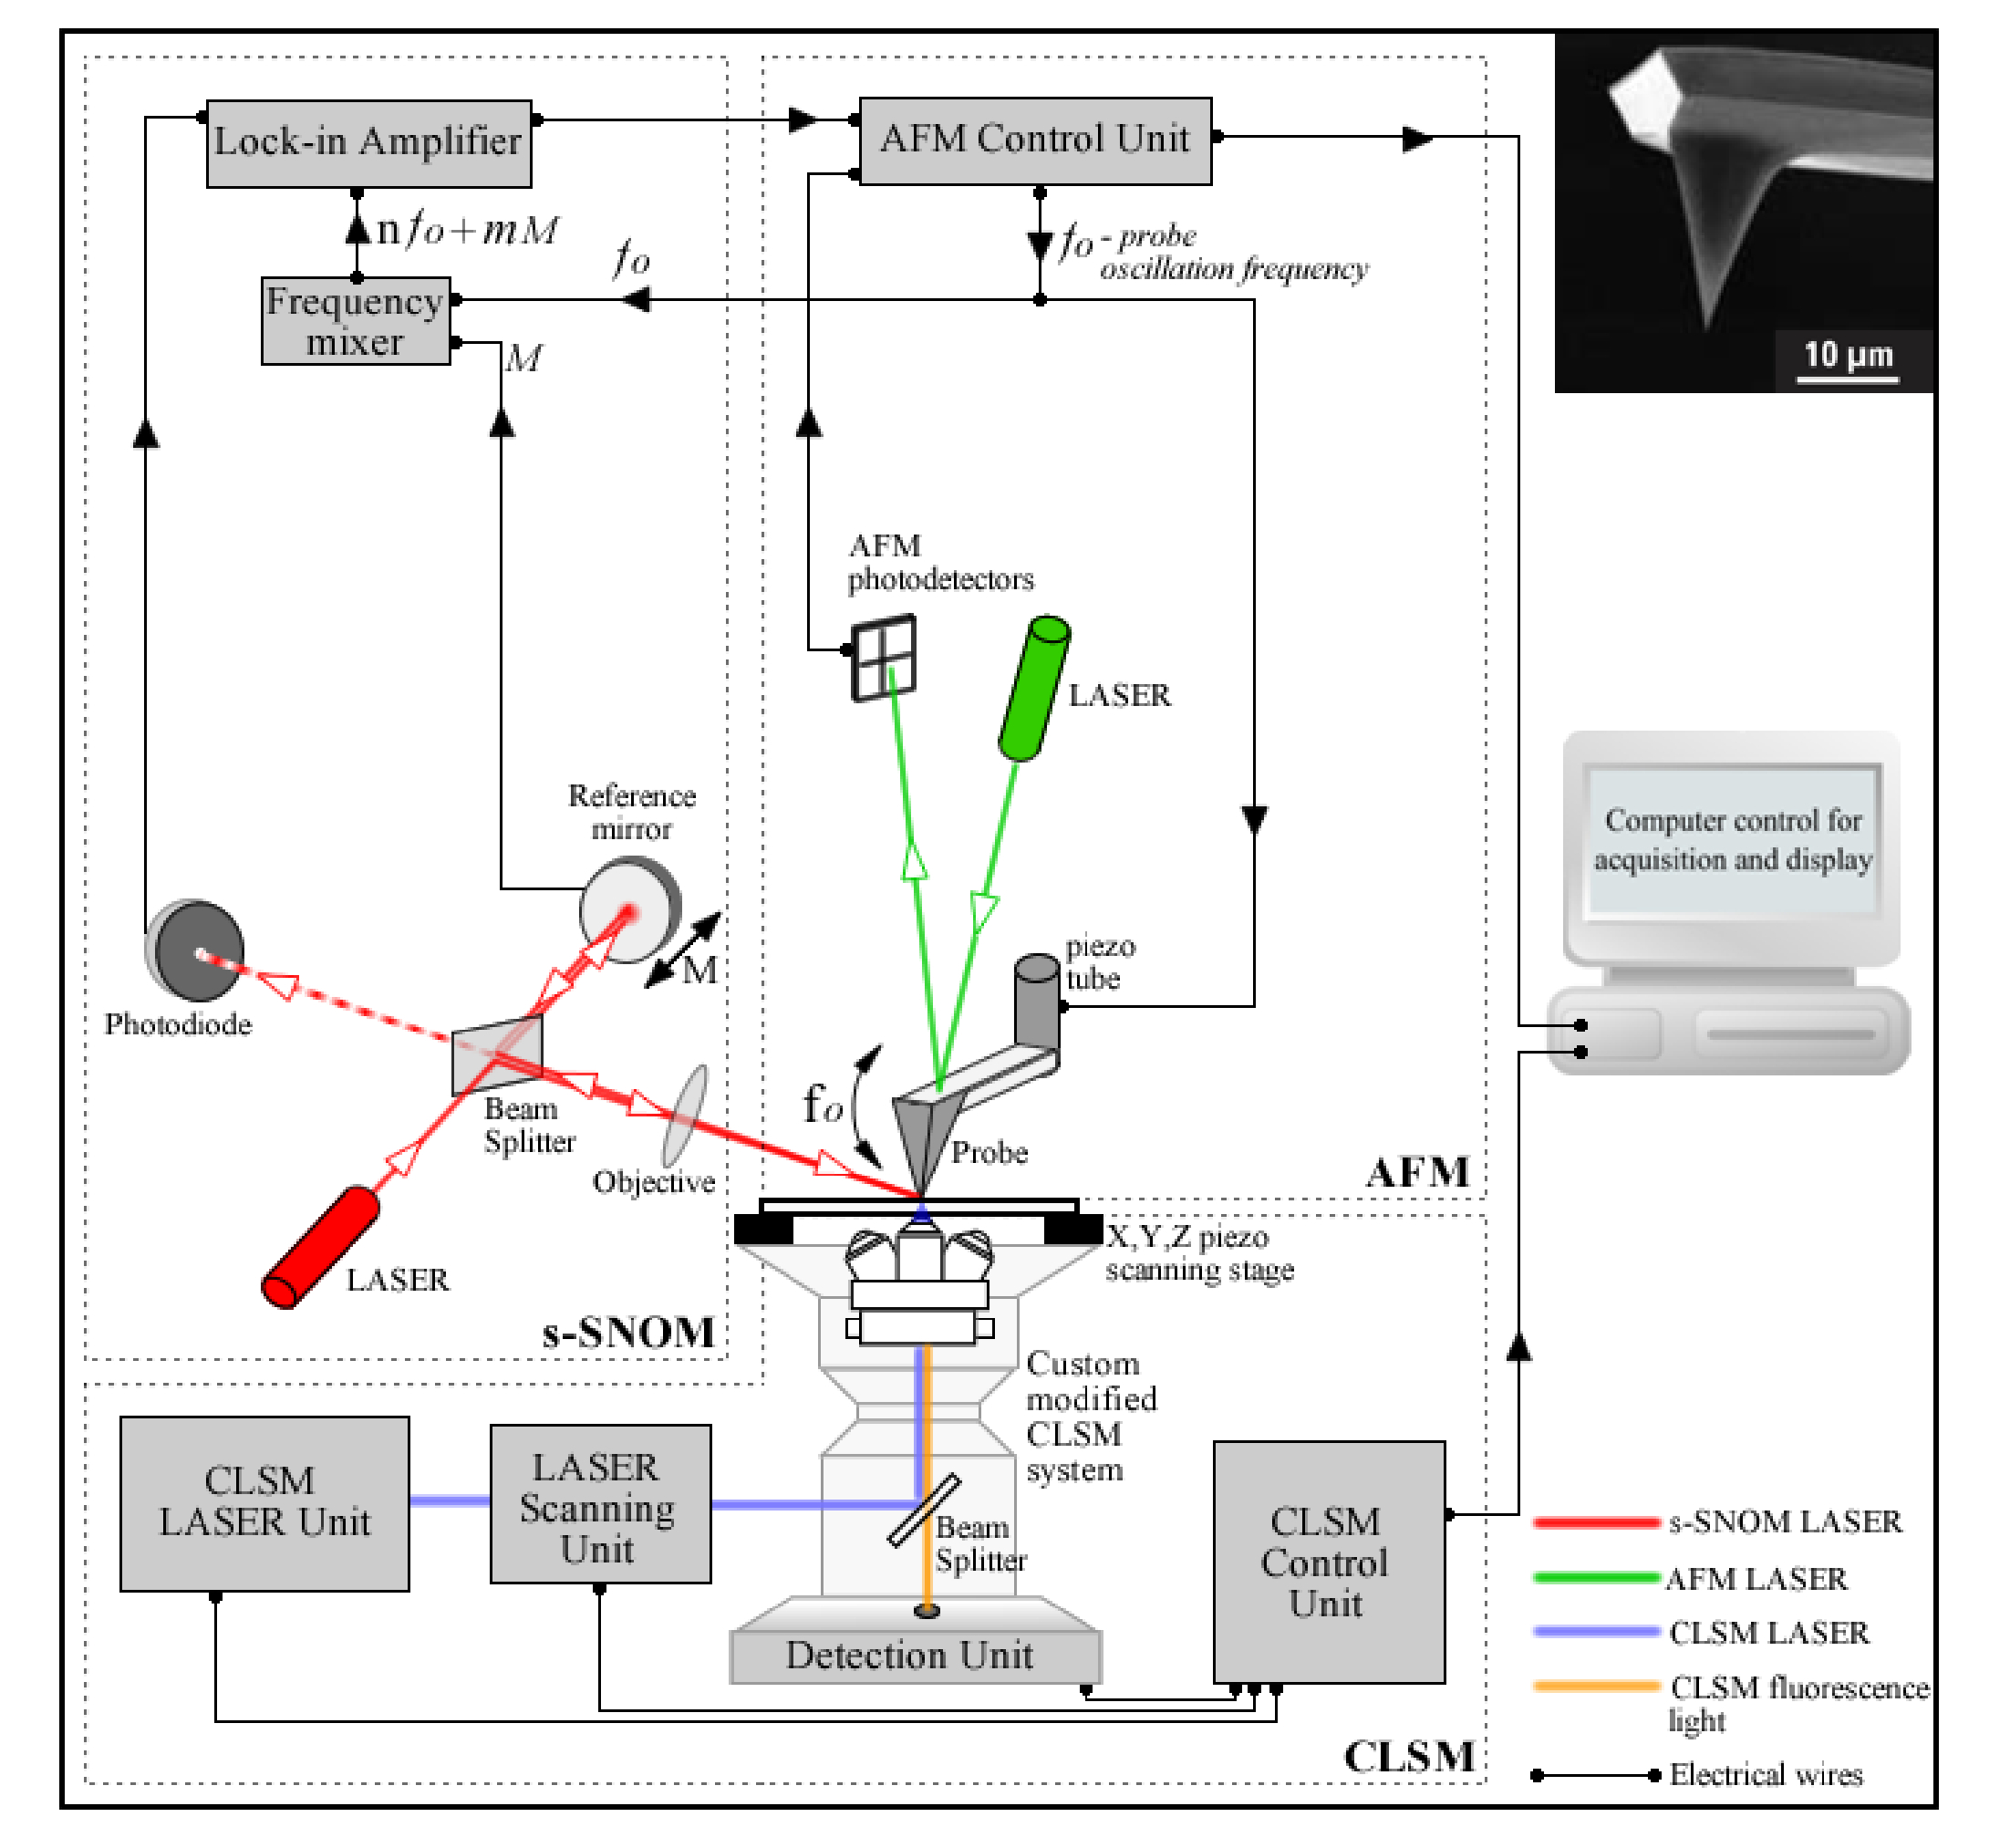
\includegraphics[keepaspectratio, height=\linewidth]{images/multimodal_system.jpg}
\caption[Sistema multimodale per l'acquisizione di immagini correlative]{
	Sistema multimodale per l'acquisizione di immagini correlative \cite{stanciu_2017}}
\label{fig:multimodal_system}
\end{figure}

\end{document}